\documentclass[xcolor={dvipsnames}, handout]{beamer}
%\documentclass[xcolor={dvipsnames}]{beamer}
\setbeamertemplate{footline}[frame number]
%\usepackage{amsmath,amsfonts,amssymb,pxfonts,eulervm,xspace}
\usepackage{amsmath, amsfonts, amssymb, mathtools, eulervm, xspace}
\renewcommand{\restriction}{\mathord{\upharpoonright}} %restriction w/p space
\usepackage{relsize}%mathlarger
\usepackage{bm}
\usepackage{centernot}
\usepackage{mathrsfs} % math script fonts
\usepackage{tikz}
\usetikzlibrary{cd} % commutative diagrams
\newtheorem{prop}{Proposition} %math?

\usepackage{subcaption} % subfigure float captioning

\usepackage{tabulary}
\usepackage{tabularx}
\usepackage{enumitem}
\usepackage{booktabs}
\usepackage{multirow}
\usepackage{array}

\usepackage{graphicx}
\usepackage{adjustbox}%scale tikz-cd

\usepackage{appendixnumberbeamer} 
\usepackage{comment}
\usepackage{minted}
\setminted[python]{fontsize=\scriptsize, 
                   linenos,
                   numbersep=8pt,
                   autogobble, 
                   frame=lines,
                   bgcolor=bg,
                   framesep=3mm} 

\usepackage{notation} % move this later

\graphicspath{.figures/}

\usepackage[backend=bibtex, sorting=none, doi=false,isbn=false,url=false, giveninits=true]{biblatex}
\bibliographystyle{plain}
\bibliography{../paper/bibliography.bib}

%\usetheme{ccnycrest}

\newenvironment{changemargin}[2]{%
\begin{list}{}{%
\setlength{\topsep}{0pt}%
\setlength{\leftmargin}{#1}%
\setlength{\rightmargin}{#2}%
\setlength{\listparindent}{\parindent}%
\setlength{\itemindent}{\parindent}%
\setleng{}th{\parsep}{\parskip}%
}%
\item[]}{\end{list}}

\begin{document}

\title{Topological Equivariant Artist Model}
\begin{comment}
\begin{frame}
	\titlepage
    Hannah Aizenman, Tom Caswell, Michael Grossberg\\
    %Committee: Dr. Robert Haralick, Dr. Lev Manovich, Dr. Huy Vo\\
    %External Member: Dr. Marcus Hanwell
\end{frame}

\section{Introduction}
\begin{frame}{What are we doing?}
    \begin{itemize}
        \item develop a model for describing data to graphic transformations
        \item specify a visualization library architecture based on this model
        \item implement functional(ish) components based on this model using ideas from functional programming
    \end{itemize}
\end{frame}

%% maybe pull out the middle for now? move the 3 stages down to construction? 
\begin{frame}{What do visualization libraries do?}
    \begin{figure}
        \begin{overprint}
            \onslide<1|handout:1>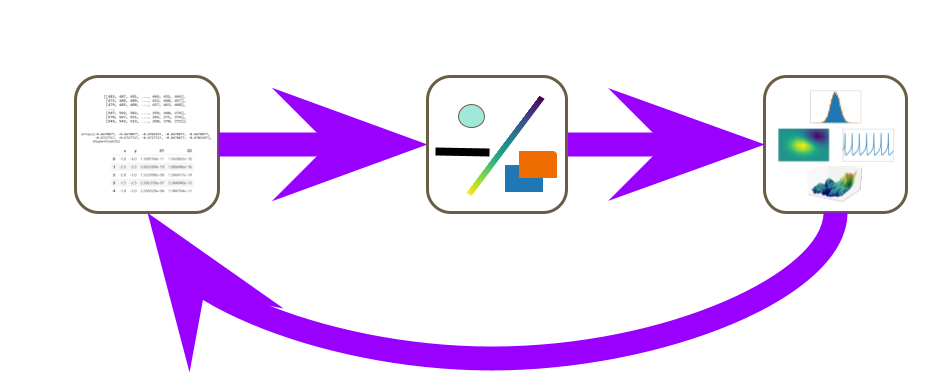
\includegraphics[width=\linewidth]{figures/flow/s2.png}
            \onslide<2|handout:2>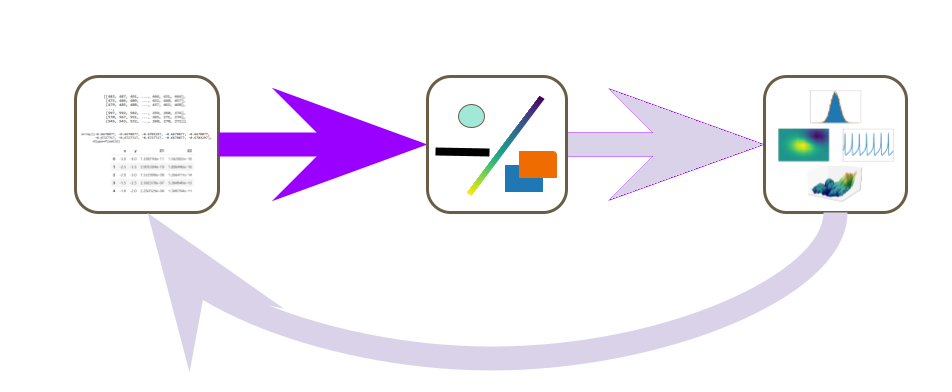
\includegraphics[width=\linewidth]{figures/flow/s_vc.png}
            \onslide<3|handout:3>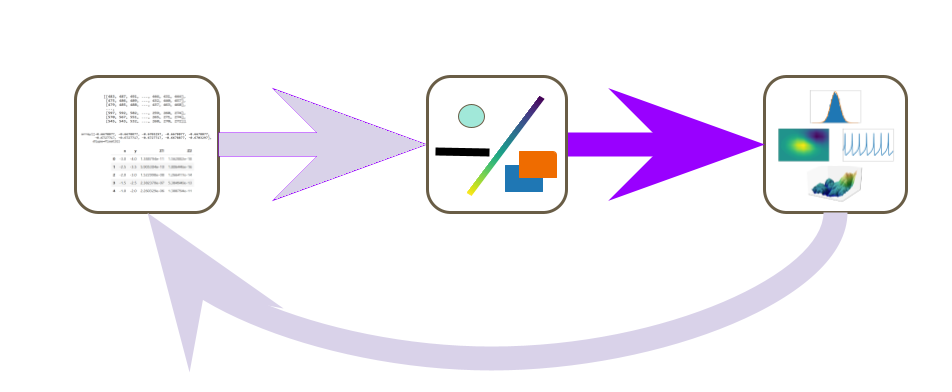
\includegraphics[width=\linewidth]{figures/flow/s_mark.png}
            \onslide<4|handout:4>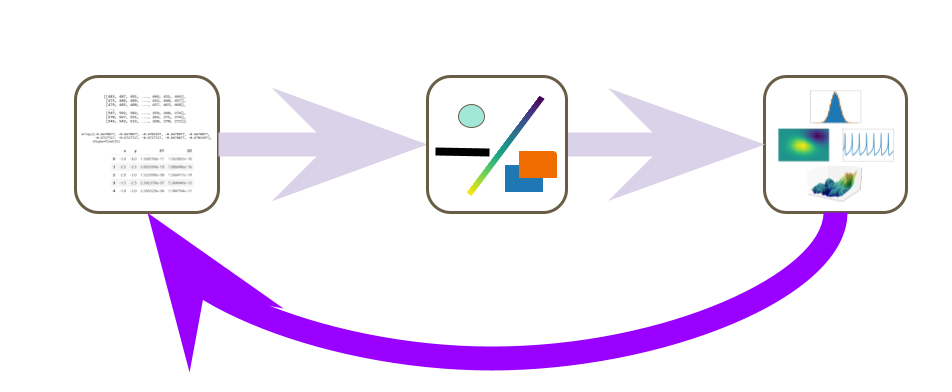
\includegraphics[width=\linewidth]{figures/flow/s3.png}
        \end{overprint}
    \end{figure}
\end{frame}

\begin{frame}{Case Study: Matplotlib}
    \begin{figure}
       
\includegraphics[width=\linewidth]{figures/flow/artists.png}
    \end{figure}
\end{frame}

\begin{frame}{Visualizations Preserve Structure}
    \begin{description}
        \item [continuity] topological properties \cite{wilkinsonGrammarGraphics2005}, i.e. how elements in a dataset are organized, e.g. discrete rows in a table, networked nodes, pixels in an image, points on a line
        \item [equivariance] data and visual encodings are matched such that transformations have an equivalent effect on data and graphical representations, e.g. rotating a matrix and image, shifting  points on a line and a line graphic
      \end{description}
\end{frame}

\begin{frame}{Continuity}
    \begin{figure}
        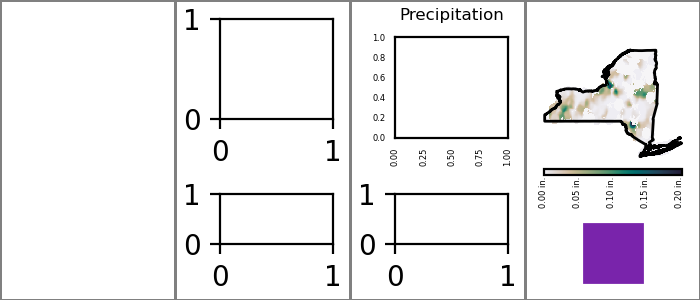
\includegraphics[width=\linewidth]{../paper/figures/k_different_types.png}
    \end{figure}
\end{frame}

\begin{frame}{Expressed in container}    
    \begin{figure}
        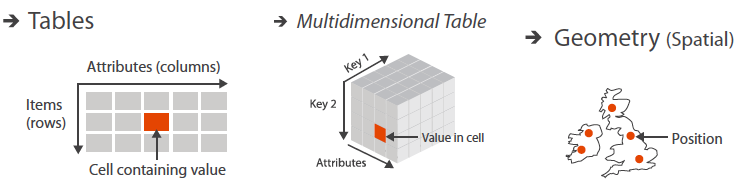
\includegraphics[width=1\textwidth]{figures/intro/munzner_datatypes.png}
        \caption{Figure 2.8 in Munzner's Visualization Analysis and Design\cite{munznerVisualizationAnalysisDesign2014}}
    \end{figure}
\end{frame}

\begin{frame}{Why is container type not enough?}
    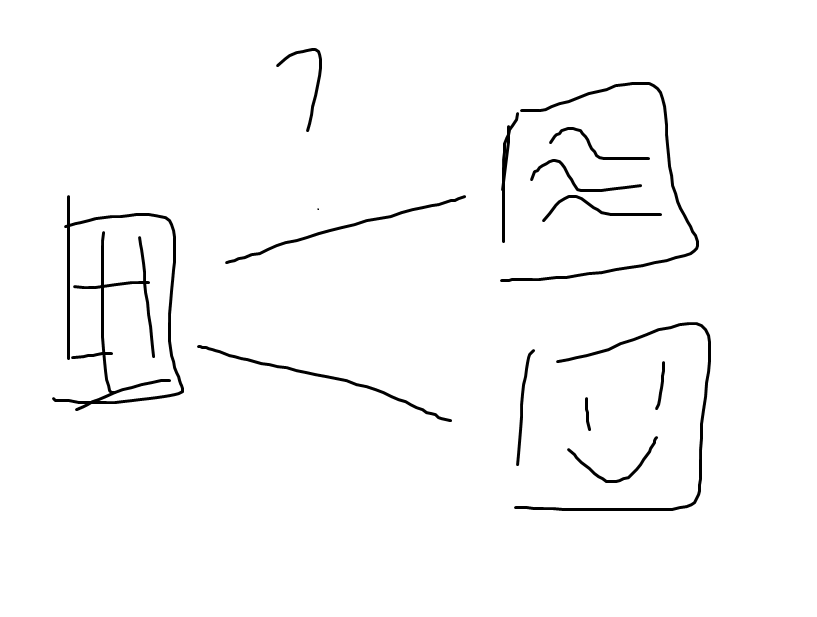
\includegraphics[width=1\linewidth]{../paper/figures/whycontinuity.png}
\end{frame}

\begin{frame}{Equivariance}
    \begin{description}
        \item[Retinal Variables \& Marks] visual encodings should match properties of the data \cite{bertinSemiologyGraphicsDiagrams2011a}
        \pause
        \item[Graphical Integrity] graphs show \textbf{only} the data\cite{tufteVisualDisplayQuantitative2001}
        \pause 
        \item[Naturalness] easier to understand when properties match\cite{norman_things_smart}
        \pause
        \item[Expressiveness] which structure preserving mappings can a tool implement\cite{mackinlayAutomatingDesignGraphical1986}] 
    \end{description}
\end{frame}

%flip columns
\begin{frame}{Frameworks for Expressing Visual Equivariance}
    \begin{description}
        \item[linguistically] visualization has syntax, semantics, grammar expresses how to design structure preserving visualizations
        \cite{mackinlayAutomatingDesignGraphical1986,mackinlayAUTOMATICDESIGNGRAPHICAL1987,wilkinsonGrammarGraphics2005}

        \item[algebraically] transformations on data and graphics are equivalent symmetric \cite{kindlmannAlgebraicProcessVisualization2014}
        \begin{columns}
            \column{.5\textwidth}
            \begin{description}
                \item[D] data 
                \item[R] data representation 
                \item[V] visualization
            \end{description}
            \column{.5\textwidth}
            \begin{equation*}
                \begin{tikzcd}[ampersand replacement=\&]
                    D \arrow[d, "\alpha"'] \arrow[r, "r_1"] \& R \arrow[r, "\nu"]  \& V \arrow[d, "\omega"] \\
                    D \arrow[r, "r_2"']                     \& R \arrow[r, "\nu"'] \& V                    
                \end{tikzcd}
                \end{equation*}
        \end{columns} 
    \item[categorically] \textit{understanding} = \textit{read} $\circ$ \textit{render} \cite{vickersUnderstandingVisualizationFormal2013}    
    \end{description}
\end{frame}

\begin{frame}{Domain specific libraries know their structure\cite{HeerSoftware2006}}
    \begin{table}
        %\renewcommand{\arraystretch}{2}
        %
        \begin{tabular}{>{\onslide<1->}l>{\onslide<2->}l>{\onslide<3->}l}
            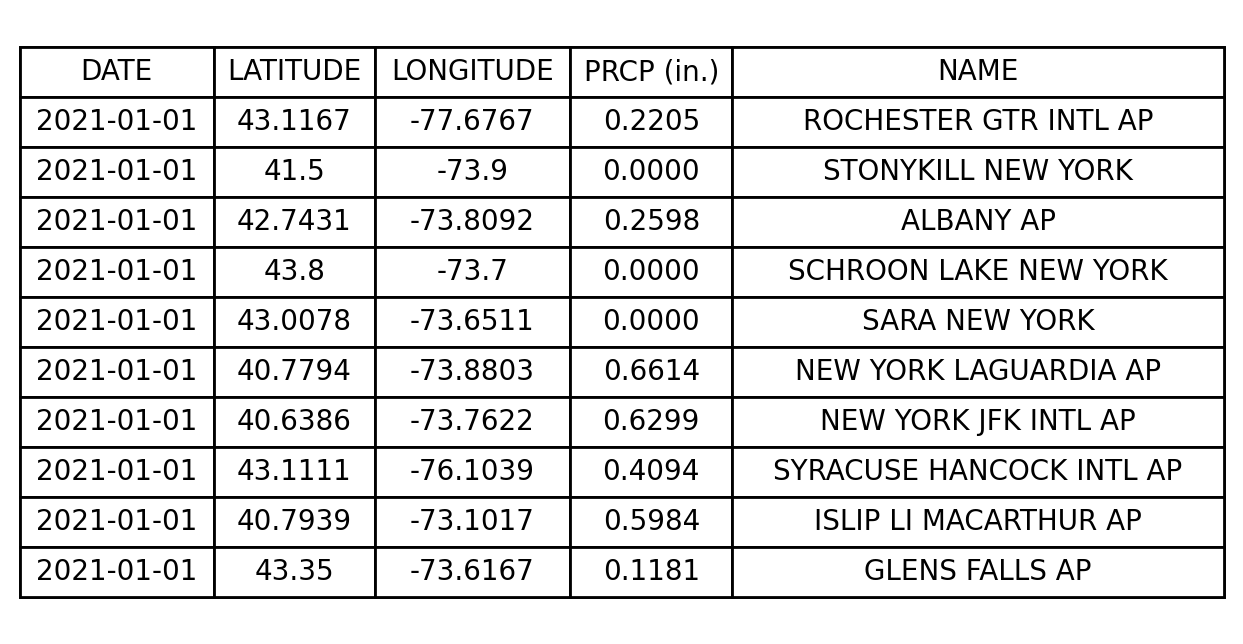
\includegraphics[width=.24\textwidth]{figures/intro/table.png} & 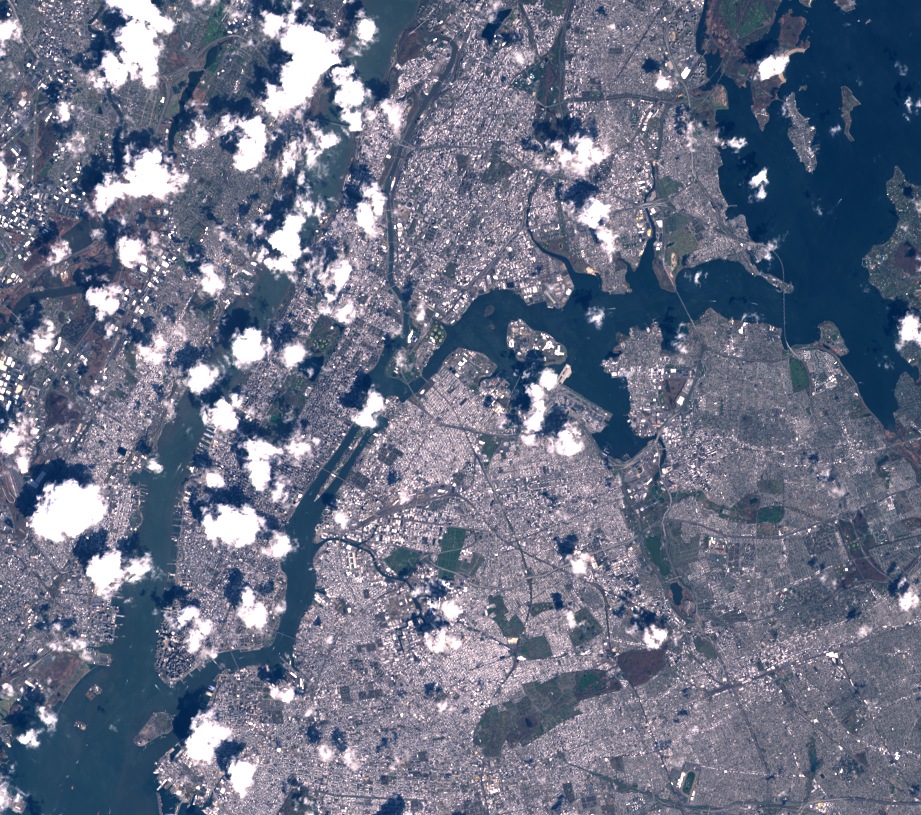
\includegraphics[width=.3\textwidth]{figures/intro/landsat.png} & 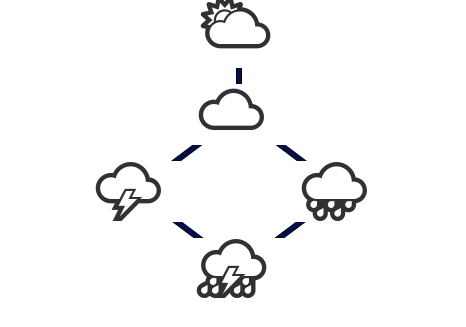
\includegraphics[width=.33\textwidth]{figures/math/graph.png} \\
            ggplot\cite{wickhamGgplot2ElegantGraphics2016a}  & ImageJ\cite{schneiderNIHImageImageJ2012}& Gephi\cite{bastianGephiOpenSource2009}\\
            Vega\cite{satyanarayanDeclarativeInteractionDesign2014} & ImagePlot\cite{studiesCulturevisImageplot2021} & Graphviz\cite{ellsonGraphvizOpenSource2002}\\
            Altair\cite{vanderplasAltairInteractiveStatistical2018}& Napari\cite{nicholas_sofroniew_2021_4533308} & Networkx\cite{HagbergExploringNetwork2008}\\
             Tableau \cite{StoltePolaris2002}& &\\
            \cite{hanrahanVizQL2006,MackinlayShowme2007}&&\\
           
        \end{tabular}
    \end{table}
\end{frame}

\begin{frame}{General purpose libraries generally can't\cite{toryRethinkingVisualizationHighlevel2004}}
    \begin{figure}
        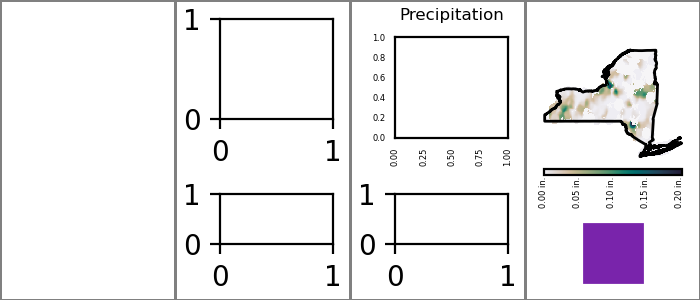
\includegraphics[height=.3\textheight]{../paper/figures/k_different_types.png}
    \end{figure}
    \begin{enumerate}
        \item Matplotlib\cite{hunterMatplotlib2DGraphics2007} $\rightarrow$Seaborn\cite{waskom2020seaborn}, xarray \cite{hoyer2017xarray} 
        \item D3 \cite{bostockDataDrivenDocuments2011}
        \item VTK \cite{hanwellVisualizationToolkitVTK2015,geveciVTK2012}(MayaVi\cite{RamachandranMayaVI2011})$\rightarrow$ Titan\cite{brianwylieUnifiedToolkitInformation2009}, ParaView\cite{ahrens2005paraview}
    \end{enumerate}
\end{frame}
\end{comment}

\section{Algebraic Topology & Category Theory}

\begin{frame}{Mathematical Data Abstraction}
    \begin{description}
        \item[Fiber Bundles] "unified, dimension-independent framework" that expresses data as the mapping between continuity and fields \cite{butlerVectorBundleClassesForm1992,butlerVisualizationModelBased1989}
        \item[Category Theory Language] express constraints in specifications \cite{wielsManagementEvolvingSpecifications1998}   
        \item[Sheaves on Bundles] "algebraic data structure" for representing data over topological spaces \cite{ghristElementaryAppliedTopology2014}
    \end{description}
\end{frame}

\begin{frame}
    \frametitle<1|handout:1>{Fiber Bundle}
    \frametitle<6|handout:2>{Data Bundle}
    \frametitle<7|handout:3>{Graphic Bundle}
    \begin{columns}
        \column{0.31\textwidth}
        \begin{equation*}
            %\label{eq:related-work:continuity:fiber-bundle}
            \begin{tikzcd}[ampersand replacement=\&, row sep=huge]
              \onslide*<3-6|handout:1-2>{\dfiberc}
              \onslide*<7|handout:3>{\gfiberc} 
              \onslide*<4-|handout:1->{\arrow[r, hook]} \& 
              \onslide*<1-6|handout:1-2>{\dtotalc} 
              \onslide*<7|handout:3>{\gtotalc}
              \onslide*<4-|handout:1->{\arrow[d, "\pi"']} \\
               \& 
               \onslide*<2-6|handout:1-2>{\dbasec}
               \onslide*<7|handout:3>{\gbasec} 
               \onslide*<5-6|handout:1-2>{\arrow[u, "\dsectionc \in \cgamma{\dbasec}{\dtotalc}"', bend right, pos=.5]}
               \onslide*<7|handout:3>{\arrow[u, "\gsectionc \in \cgamma{\gbasec}{\gtotalc}"', bend right, pos=.5]}
            \end{tikzcd}
        \end{equation*}
     \column{0.69\textwidth}
     \only<1-5|handout:1>{
        \begin{description}[style=nextline]
            \item<1-5|handout:1>[\textcolor{total}{Total Space}]{$(\dtotalc, \mathcal{T}_{\dtotalc})$}
            \item<2-5|handout:1>[\textcolor{base}{Base Space}]{$(\dbasec, \mathcal{T}_{\dbasec}),\; \dbasepointc \in \opensetc \subseteq \dbasec$}
            \item<3-5|handout:1>[\textcolor{fiber}{Fiber Space}]{$\dfiberc\restriction_{\dbasepointc} = \pi^{-1}(\dbasepointc), \dfiberc = \dfiberc\restriction_{\dbasepointc}\; \forall \dbasepointc \in \dbasec$}
        \end{description}
        }
    \only<6|handout:2>{
        \begin{description}[style=nextline]
            \item[\textcolor{total}{Data \dtotalc}]{continuity + fields}
            \item[\textcolor{base}{Continuity \dbasec}]{how data elements are organized (topological properties) \cite{wilkinsonGrammarGraphics2005}, index (key) space \cite{munznerWhatDataAbstraction2014})}
            \item[\textcolor{fiber}{Fields \dfiberc}] {generalization of a schema - named and typed date fields \cite{spivakSIMPLICIALDATABASES, spivakDatabasesAreCategories2010}}
        \end{description}
        }
        \only<7|handout:3>{
            \begin{description}[style=nextline]
                \item[\textcolor{total}{Graphic \gtotalc}]{continuity + renderer fields}
                \item[\textcolor{base}{Continuity \gbasec}]{parameterization of the graphic's geometry}
                \item[\textcolor{fiber}{Display \gfiberc}] {renderer fields, e.g. \{xy,rgba\}, \{xy, cymk\}, \{xyz, rgba\}}
            \end{description}
            }
    \end{columns}
    \pause 
    \only<4-5|handout:1>{
        \begin{alertblock}{}
            \begin{description}[style=nextline]
                \item[\textcolor{section}{Sections}]{$\cgamma{\opensetc}{\dtotalc\restriction_{\opensetc}} \coloneqq \big\{\dsectionc: \opensetc\rightarrow \dtotalc\restriction_{\opensetc} \; \bigm{\vert} \pi(\dsectionc(\dbasepointc)) = \dbasepointc\;for\, all\; \dbasepointc \in \opensetc \big\}$}
                \item[Locally Trivial] {for every point $\dbasepointc \in \dbasec$, there exists an open neighborhood $\dbasepointc \in \opensetc \subseteq \dbasec$ s.t. there is a homeomorphism $\pi^{-1}(\opensetc)\xrightarrow{\varphi} \opensetc \times \dfiberc$}
                \item[(Globally) Trivial]{$\dtotalc = \dbasec \times \dfiberc$}
            \end{description}
        \end{alertblock}
    }
    \only<6|handout:2>{
    \begin{alertblock}{}
        \begin{description}[style=nextline]
            \item[\textcolor{section}{Data} \cite{butlerVisualizationModelBased1989,butlerVectorBundleClassesForm1992}]{$
        \dsectionc(\dbasepointc) = \;\delementc,\; \dbasepointc\in \opensetc \subseteq \dbasec,\; \delementc \in \dfiberc\restriction_{\dbasepointc}$} 
        \item[]{$\delementc=\{field_0:value, \cdots field_i:value, \cdots field_n:value\}$}
        \end{description}
    \end{alertblock}
    }
    \only<7|handout:3>{
        \begin{alertblock}{}
            \begin{description}[style=nextline]
                \item[\textcolor{section}{Graphic}]{$\cgamma{\opensetgc}{\gtotalc\restriction_{\opensetgc}} \coloneqq \big\{\gsectionc: \opensetgc\rightarrow \gtotalc\restriction_{\opensetgc} \; \bigm{\vert} \pi(\gsectionc(\gbasepointc)) = \gbasepointc\;for\, all\; \gbasepointc \in \opensetgc \big\}$}
                \item[] {$\gsectionc(\gbasepointc) = \gelementc,\; \gbasepointc\in \opensetgc\subseteq \gbasec,\; \gelementc \in \dfiberc\restriction_{\gbasepointc}$}
                \item[] $\gelementc=\{x,\,y,\,r,\,g,\,b\}$
           
        \end{description}    
    \end{alertblock}
    }
\end{frame}

\subsection{Category Theory}
\begin{frame}[fragile]{}
    \begin{minted}{python}
        Artist(data:Data) -> Graphic
    \end{minted}
\end{frame}

\begin{frame}{Category $\textcolor{source}{\mathcal{C}}$}
\begin{columns}
    \column{0.39\textwidth}
    \begin{equation*}
    \begin{tikzcd}[ampersand replacement=\&]
        \onslide*<1-|handout:1>{\textcolor{source}{C_1}} 
        \onslide*<3-|handout:1>{\arrow[r, "f", color=source]}
        \onslide*<4-|handout:1>{\arrow[rd, "g\circ f"', color=source]}
        \onslide*<2-|handout:1>{\arrow["id_{C_1}"', loop, distance=2em, in=215, out=145, color=source]} \& 
        \onslide*<1-|handout:1>{\textcolor{source}{C_2}}
        \onslide*<3-|handout:1>{\arrow[d, "g", color=source]} 
        \onslide*<2-|handout:1>{\arrow["id_{C_2}"', loop, distance=2em, in=125, out=55, color=source]} \\\& 
        \onslide*<1-|handout:1>{\textcolor{source}{C_3}}
        \onslide*<2-|handout:1>{\arrow["id_{C_3}"', loop, distance=2em, in=305, out=235, color=source]}              
    \end{tikzcd}
    \end{equation*}
    \column{0.59\textwidth}
    \begin{alertblock}<5-|handout:1>{associativity} 
        if $f: C_1 \rightarrow C_2$, $g: C_2 \rightarrow C_3$ and $h: C_3 \rightarrow C_4$ then $h\circ (g \circ f) = (h \circ g) \circ f$
    \end{alertblock}
    \begin{alertblock}<6-|handout:1>{identity} 
        for every $f: C_1 \rightarrow C_2$ there exists identity morphisms $f \circ id_{C_1} = f = id_{C_2} \circ f$
    \end{alertblock}
    \end{columns}
\end{frame}


\begin{frame}{Opposite Category $\textcolor{source}{\mathcal{C}^{op}}$}
    \begin{columns}
        \column{0.49\textwidth}
    \begin{equation*}
        \begin{tikzcd}[ampersand replacement=\&]
            \textcolor{fade}{C_1} \arrow[r, "f", color=fade] \arrow[rd, "g\circ f"', color=fade] \arrow["id_{C_1}"', loop, distance=2em, in=215, out=145, color=fade] \& \textcolor{fade}{C_2} \arrow[d, "g", color=fade] \arrow["id_{C_2}"', loop, distance=2em, in=125, out=55, color=fade] \\
        \& \textcolor{fade}{C_3} \arrow["id_{C_3}"', loop, distance=2em, in=305, out=235, color=fade]              
        \end{tikzcd}
        \end{equation*}
        \column{0.49\textwidth}
        \begin{equation*}
        \begin{tikzcd}[ampersand replacement = \&]
            \textcolor{source}{C_1} \arrow["id_{C_1}"', loop, distance=2em, in=215, out=145, color=source] \& \textcolor{source}{C_2} \arrow[l, "f"',color=source] \arrow["id_{C_2}"', loop, distance=2em, in=125, out=55, color=source]\\
            \& \textcolor{source}{C_3} \arrow[u, "g"', color=source] \arrow[lu, "f \circ g", color=source] \arrow["id_{C_3}"', loop, distance=2em, in=305, out=235, color=source]
            \end{tikzcd}
        \end{equation*}
        \end{columns}
\end{frame}

\begin{frame}{Functor $\textcolor{functor}{\bm{F}}: \textcolor{source}{\mathcal{C}} \rightarrow \textcolor{target}{\mathcal{D}}$}
\begin{columns}
    \column{.39\textwidth}
    \begin{equation*}
        \begin{tikzcd}[ampersand replacement = \&, ]
            \onslide*<1-|handout:1>{\textcolor{source}{c}} 
            \onslide*<1-|handout:1>{\arrow[d, "f"', shift right=0, color=source]} 
            \onslide*<3-|handout:1>{\arrow[r, "F", color=functor, maps to]} \& 
            \onslide*<2-3|handout:0>{\textcolor{target}{d}}
            \onslide*<4-|handout:0>{\textcolor{target}{F(c)}} 
            \onslide*<0|handout:1>{\textcolor{target}{F(c)=d}} 
            \onslide*<2|handout:0>{\arrow[d, shift right=0, color=target]}
            \onslide*<3-|handout:0>{\arrow[d, "F(f)", shift right=0, color=target]}
            \onslide*<0|handout:1>{\arrow[d, "F(f)", shift right=3, color=target]} \\
            \onslide*<1-|handout:1>{\textcolor{source}{c^{\prime}}} 
            \onslide*<3-|handout:1>{\arrow[r, "F"', color=functor, maps to]}\& 
            \onslide*<2-3|handout:0>{\textcolor{target}{d^{\prime}}}
            \onslide*<4-|handout:0>{\textcolor{target}{F(c^{\prime})}}
            \onslide*<0|handout:1>{\textcolor{target}{F(c^{\prime})= d^{\prime}}}                    
        \end{tikzcd}
    \end{equation*}
    \column{.59\textwidth}
    \begin{alertblock}<5-|handout:1>{composition}
        \begin{align*}
            \textcolor{functor}{F}(\textcolor{source}{g}) \circ  \textcolor{functor}{F}(\textcolor{source}{f}) = \textcolor{functor}{F} (\textcolor{source}{g}\circ \textcolor{source}{f})
        \end{align*}
    \end{alertblock}
    \begin{alertblock}<6-|handout:1>{identity}
        \begin{align*}
            \textcolor{functor}{F}(\textcolor{source}{id_c}) = \textcolor{target}{id}_{\textcolor{functor}{F}(\textcolor{source}{c})}
        \end{align*}
    \end{alertblock}
\end{columns}
\end{frame}

\begin{frame}{Presheaf: $\sheafc: \mathcal{C}^{op} \textcolor{sheaf}{\rightarrow} \setc $}
    \begin{columns}
    \column{0.29\textwidth}
    \begin{tikzcd}[ampersand replacement=\&, row sep=huge]
        \onslide*<9-|handout:1->{\dfiberc}
        \onslide*<9-|handout:1->{\arrow[r, hook]} \& 
        \onslide*<1-|handout:1->{\dtotalc}
        \onslide*<1-|handout:1->{\arrow[d, "\pi"']} \\
           \& 
        \onslide*<1-|handout:1->{\dbasec}
        \onslide*<3-|handout:1->{\arrow[u, "\dsectionc \in \cgamma{\dbasec}{\dtotalc}"', bend right, pos=.5]}
        \end{tikzcd}
    \column{0.69\textwidth}
        \begin{tikzcd}[ampersand replacement = \&, column sep=small]
            \onslide*<3,6-|handout:0>{{\cgamma{\opensetc_1}{\dtotalc\restriction_{{\opensetc_1}}}}} 
            \onslide*<4-5|handout:0>{{\cgamma{\opensetc_1}{\dtotalc\restriction_{{\opensetc_1}}}}\in \setc}
            \onslide*<0|handout:1>{\setc \ni {\cgamma{\opensetc_1}{\dtotalc\restriction_{{\opensetc_1}}}}}
            \&  
            {} \& 
            \onslide*<6-|handout:1>{{\cgamma{\opensetc_2}{\dtotalc\restriction_{\opensetc_2}}}} 
            \onslide*<7-|handout:1>{\arrow[ll, "\iota^*"', hook', color=set]} \\\& \&\\
            \onslide*<3|handout:0>{\opensetc_1 \subset \dbasec}
            \onslide*<4-5|handout:0>{\opensetc_1 \in Ob(\mathcal{\dbasec}^{\textcolor{base}{op}})}
            \onslide*<6-|handout:0>{\opensetc_1}
            \onslide*<0|handout:1>{Ob(\mathcal{\dbasec}^{\textcolor{base}{op}}) \ni \opensetc_1} 
            \onslide*<5-|handout:0>{\arrow[uu, "\sheafc_{\dbasec, \dtotalc}", maps to, color=sheaf]}
            \onslide*<0|handout:1>{\arrow[uu, "\sheafc_{\dbasec, \dtotalc}", maps to, color=sheaf, shift right = 10]}
            \onslide*<7-|handout:1>{\arrow[rr, "\iota"', hook, color=base]} \&   
            \onslide*<8-|handout:1>{\arrow[uu, "\sheafc_{\dbasec, \dtotalc}" description, maps to, color=sheaf]} \& 
            \onslide*<6-|handout:1>{\opensetc_2} 
            \onslide*<6-|handout:1>{\arrow[uu, "\sheafc_{\dbasec, \dtotalc}"', maps to, color=sheaf]}                   
            \end{tikzcd}
    \end{columns}
    \begin{center}
        \begin{alertblock}<8-|handout:1>{stalk}
            \begin{align*}
                \sheafc_{\dbasec, \dtotalc}\restriction_{\dbasepointc}\coloneqq \lim\limits_{\opensetc\ni \dbasepointc} \Gamma(\opensetc, \dtotalc\restriction_{\opensetc}) \\
                 \dfiberc_{\dbasepointc} \subset  \sheafc_{\dbasec, \dtotalc}\restriction_{\dbasepointc}
            \end{align*}
        \end{alertblock}

        \begin{alertblock}<9-|handout:1>{germ}
            %germ  is tau at limit, \tau(k) \in germ
            \begin{align*}
                \dsectionc(\dbasepointc) \in \sheafc_{\dbasec, \dtotalc}\restriction_{\dbasepointc}
            \end{align*}
        \end{alertblock}
    \end{center}
\end{frame}


\begin{frame}{Sheaves} 
    A sheaf is a presheaf that satisfies the following two axioms\cite{bakerMathsSheaf}\\
    \begin{block}<2-|handout:1>{locality}
        if there exists the open covering $\mathcal{\opensetc} = \{\opensetc_i\}_{i\in I}$ of \opensetc
        \onslide<3-|handout:1>{
        and if $\dsectionc^{a}, \dsectionc^{b} \in \sheafc(\opensetc_i)$ have the property $\dsectionc^{a}\restriction_{\opensetc_i} = \dsectionc^{b}\restriction_{\opensetc_i}$ for each $\opensetc_i \in \mathcal{\opensetc}$,}
        \onslide<4|handout:1>{ then $\dsectionc^{a} = \dsectionc^{b}$}
    \end{block} 
    \begin{block}<5-|handout:1>{gluing} 
        if there exists the open covering $\mathcal{\opensetc} = \{\opensetc_i\}_{i\in I}$ of \opensetc\ and if $\dsectionc^{i} \in \sheafc(\opensetc_i)$ is given for each $i \in I$
        \onslide<6-|handout:1>{such that ${\dsectionc^{i}}\restriction_{\opensetc_i\cap \opensetc_j} = {\dsectionc^{j}}\restriction_{\opensetc_i \cap \opensetc_j}$ for each pair $\opensetc_i, \opensetc_j \in \mathcal{\opensetc}$,}
        \onslide<7-|handout:1>{ then there exists $\dsectionc \in \sheafc(\opensetc)$ such that $\dsectionc\restriction_{\opensetc_i} = {\dsectionc^{i}}$ for each $i \in I$} 
    \end{block}      
\end{frame}

\begin{frame}
    \frametitle<3|handout:3>{Functor: $\vindexc: \mathcal{\gbasec} \rightarrow \mathcal{\dbasec}$}
    \frametitle<1|handout:1>{Data}
    \frametitle<4-6|handout:4>{Pullback: data to region of the visualization} 
    \frametitle<2|handout:2>{Graphic}
    \frametitle<7-|handout:5>{Pushforward: visualization to index of data}
    \begin{equation*}
        \begin{tikzcd}[ampersand replacement=\&, row sep=huge]
            \onslide*<0|handout:2,3,5>{\sheafc_{\gbasec, \gtotalc}} 
            \onslide*<0|handout:5>{\arrow[rr, "\textcolor{functor}{\vindexpush}", color=functor]} \& \& 
            \onslide*<0|handout:5>{\textcolor{functor}{\vindexpush}\sheafc_{\gbasec, \gtotalc}}  
            \\
            \onslide*<0|handout:2->{\gbasec}
            \onslide*<0|handout:3->{\arrow[rr, "\vindex", color=functor]}
            \onslide*<0|handout:2,3,5>{\arrow[u, "\sheaf_{\gbasec, \gtotalc}", maps to, color=sheaf]}
            \onslide*<0|handout:4>{\arrow[d, dashed, maps to, color=sheaf]} \&  \& 
            \onslide*<0|handout:1,3->{\dbasec}
            \onslide*<0|handout:1,3-4>{\arrow[d, "\sheaf_{\dbasec, \dtotalc}", maps to, color=sheaf]}
            \onslide*<0|handout:5>{\arrow[u, dashed, maps to, color=sheaf]} \\
            \onslide*<0|handout:4>{\textcolor{functor}{\vindexpull}\sheafc_{\dbasec, \dtotalc}} 
             \& \& 
            \onslide*<0|handout:1,3-4>{\sheafc_{\dbasec, \dtotalc}}
            \onslide*<0|handout:4>{\arrow[ll, "\textcolor{functor}{\vindexpull}", color=functor]} 
        \end{tikzcd}
    \end{equation*}
    \only<0|handout:1>{
        \begin{itemize}
            \item $\dfiberc \hookrightarrow \dtotalc \xrightarrow{\pi} \dbasec$
            \item $\sheafc_{\dbasec, \dtotalc}:\opensetc \mapsto \cgamma{\opensetc}{\dtotalc\restriction_{\opensetc}}, \opensetc \subset \dbasec$
            \item $\cgamma{\opensetc}{\dtotalc\restriction_{\opensetc}} \ni \dsectionc: \opensetc \rightarrow \dfiberc\restriction_{\opensetc}$
            \item $\dsectionc(\dbasepointc) = \{f_0:v_0, \cdots,\}, \dbasepointc \in \opensetc$
        \end{itemize}
    }
    \only<0|handout:4>{
        \begin{itemize}
            \item $\vindexpullc\dfiberc \hookrightarrow \vindexpullc\dtotalc \xrightarrow{\pi} \gbasec$
            \item $\vindexpullc\sheafc_{\dbasec,\dtotalc}:\opensetgc \mapsto \cgamma{\opensetgc}{\vindexpullc\dtotalc\restriction_{\opensetgc}}, \opensetgc \subset \gbasec$
            \item $\cgamma{\opensetgc}{\vindexpullc\dtotalc\restriction_{\opensetgc}} \ni \vindexpullc\dsectionc: \opensetgc \rightarrow \vindexpullc\dfiberc\restriction_{\opensetgc}$
            \item $\vindexpullc\dsectionc(\gbasepointc) = \dsectionc(\vindexc(\gbasepointc)) = \dsectionc(\dbasepointc)$
        \end{itemize}
    }
    \only<0|handout:2>{
        \begin{itemize}
            \item $\gfiberc \hookrightarrow \gtotalc \xrightarrow{\pi} \gbasec$
            \item $\sheafc_{\gbasec, \gtotalc}:\opensetgc \mapsto \cgamma{\opensetgc}{\dtotalc\restriction_{\opensetgc}}, \opensetgc \subset \gbasec$
            \item $\cgamma{\opensetgc}{\gtotalc\restriction_{\opensetgc}} \ni \gsectionc: \opensetgc \rightarrow \gfiberc\restriction_{\opensetgc}$
            \item $\gsectionc(\gbasepointc) = \{d_0, \cdots\}, \gbasepointc \in \opensetgc$
        \end{itemize}
    }
    \only<0|handout:5>{
        \begin{itemize}
            \item $\vindexpushc\gfiberc \hookrightarrow \vindexpushc\gtotalc \xrightarrow{\pi} \dbasec$
            \item $\vindexpushc\sheafc_{\gbasec, \gtotalc}:\opensetc \mapsto \cgamma{\opensetc}{\vindexpushc\gtotalc\restriction_{\opensetc}}, \opensetc \subset \dbasec$
            \item $\cgamma{\opensetc}{\gtotalc\restriction_{\opensetc}} \ni \gsectionc: \opensetc \rightarrow \gfiberc\restriction_{\opensetc}$
            \item $\vindexpushc\gsectionc(\gbasepointc) = \gsectionc\restriction_{\vindexpre(\dbasepointc)} = \gsectionc(\gbasepointc) \forall \gbasepointc \in \vindexpre(\dbasepointc)$ 
        \end{itemize}
    }
\end{frame}


%add transition slide->possibly call back 
\begin{frame}
    {\huge
        \begin{equation*}
            \sheafc_{\dbasec,\dtotalc} \textcolor{artist}{\xrightarrow{\vartistc}} \sheafc_{\gbasec, \gtotalc}
        \end{equation*}
    }
\end{frame}

\begin{frame}{Natural Transformation $\textcolor{nattran}{\alpha}: \textcolor{functor}{F} \textcolor{nattran}{\Rightarrow} \textcolor{functor}{G}$}

    \adjustbox{scale=3, center}{
        \begin{tikzcd}[ampersand replacement=\&]
            \& {} \arrow[dd, "\alpha" , Rightarrow, shorten=1.5em, color=nattran] \&             \\
          \textcolor{source}{\mathcal{C}} \arrow[rr, "F", bend left, color=functor, maps to] \arrow[rr, "G"', bend right, color=functor, maps to] \& \& \textcolor{target}{\mathcal{D}} \\
            \& {} \&            
          \end{tikzcd}}
\end{frame}
    
\begin{frame}{Natural Transformation $\textcolor{nattran}{\alpha}: \textcolor{functor}{F} \textcolor{nattran}{\Rightarrow} \textcolor{functor}{G}$}
    \begin{equation*}
        \begin{tikzcd}[column sep=huge, ampersand replacement = \&]
            \onslide*<2-|handout:1>{\textcolor{target}{F(c)}}
            \onslide*<2-|handout:1>{\arrow[dd, "F(f)"', color=target]}
            \onslide*<4-5|handout:1>{\arrow[rr, "\alpha_{c}", bend left, color=nattran, Rightarrow]}  
            \onslide*<6|handout:0>{\arrow[rr, "\alpha_{c}", color=nattran, Rightarrow]} \& 
            \onslide*<1-4|handout:1>{\textcolor{source}{c}} 
            \onslide*<1-4|handout:1>{\arrow[dd, "f" description, color=source]}
            \onslide*<3-4|handout:1>{\arrow[r, "G"', color=functor,maps to ]}
            \onslide*<2-4|handout:1>{\arrow[l, "F", color=functor, maps to]} \& 
            \onslide*<3-|handout:1>{\textcolor{target}{G(c)}} 
            \onslide*<3-|handout:1>{\arrow[dd, "G(f)", color=target, maps to]} \\
            {} 
            \onslide*<4|handout:1>{\arrow[rr, dotted, color=nattran, Rightarrow]}
            \onslide*<5|handout:0>{\arrow[rr, color=nattran, Rightarrow]} \& \& {}                      \\
            \onslide*<2-|handout:1>{\textcolor{target}{F(c^{\prime})}} 
            \onslide*<4-5|handout:1>{\arrow[rr, "\alpha_{c^{\prime}}"', bend right, color=nattran, Rightarrow]} 
            \onslide*<4-5|handout:0>{\arrow[rr, "\alpha_{c^{\prime}}"', color=nattran, maps to]}\& 
            \onslide*<1-4|handout:1>{\textcolor{source}{c^{\prime}}}
            \onslide*<2-4|handout:1>{\arrow[l, "F"', color=functor, maps to]} 
            \onslide*<3-4|handout:1>{\arrow[r, "G", color=functor, maps to]} \& 
            \onslide*<3-|handout:1>{\textcolor{target}{G(c^{\prime})}}          
        \end{tikzcd}
    \end{equation*}    
\end{frame}


\begin{frame}
    \frametitle<1-2|handout:1>{Data Space: $\vartistc_{\opensetc}: \sheafc_{\dbasec, \dtotalc} \textcolor{artist}{\Rightarrow} \vindexpushc\sheafc_{\gbasec, \gtotalc}$}
    \frametitle<3-4|handout:2>{Display Space: $\vartist_{\opensetgc}: \vindexpullc\sheafc_{\dbasec, \dtotalc} \textcolor{artist}{\Rightarrow} \sheafc_{\gbasec, \gtotalc}$}
    \frametitle<5|handout:3->{\textcolor{artist}{Artist} \vartistc}

    \onslide*<1|handout:1>{
        \begin{equation*}
      \begin{tikzcd}[ampersand replacement =\&]
        \cgamma{\opensetc_1}{\dtotalc} 
        \arrow[dd, "\iota^*"', hook, color=set] 
        \arrow[rrrr, "\vartistc_{\opensetc_1}", bend left, color=artist, Rightarrow] \&  \& 
        \opensetc_1 
        \arrow[ll, "\sheafc_{\dtotalc}", color=sheaf, maps to] 
        \arrow[rr, "\sheafc_{\gtotalpushc}"', color=sheaf, maps to] \&  \& 
        \cgamma{\opensetc_1}{\gtotalpushc} 
        \arrow[dd, "\iota^*", hook', color=set] \\
        {} 
        \arrow[rrrr, dotted, color=artist,Rightarrow] \&\&\&\& {} \\
        \cgamma{\opensetc_2}{\dtotalc} 
        \arrow[rrrr, "\vartistc_{\opensetc_2}"', bend right, color=artist, Rightarrow] \&  \& 
        \opensetc_2 
        \arrow[ll, "\sheafc_{\dtotalc}"', color=sheaf, maps to] 
        \arrow[rr, "\sheafc_{\gtotalpushc}", color=sheaf, maps to] 
        \arrow[uu, "\iota" description, hook, color=base] \& \& 
        \cgamma{\opensetc_2}{\gtotalpushc}               
    \end{tikzcd}
        \end{equation*}}

    \onslide*<0|handout:2>{
        \begin{equation*}
    \begin{tikzcd}[ampersand replacement =\&]
    \cgamma{\opensetgc_1}{\dtotalpullc} 
    \arrow[dd, "\iota^*"', hook, color=set] 
    \arrow[rrrr, "\vartistc_{\opensetgc_1}", bend left, color=artist, Rightarrow] \&  \& 
    \opensetgc_1 
    \arrow[ll, "\sheafc_{\dtotalpullc}", color=sheaf, maps to] 
    \arrow[rr, "\sheafc_{\gtotalc}"', color=sheaf, maps to] \&  \& 
    \cgamma{\opensetgc_1}{\gtotalc} 
    \arrow[dd, "\iota^*", hook', color=set] \\
    {} 
    \arrow[rrrr, dotted, color=artist, Rightarrow] \&\&\&\& {} \\
    \cgamma{\opensetgc_2}{\dtotalpullc} 
    \arrow[rrrr, "\vartistc_{\opensetgc_2}"', bend right, color=artist, Rightarrow] \&  \& 
    \opensetgc_2 
    \arrow[ll, "\sheafc_{\dtotalpullc}"', color=sheaf, maps to] 
    \arrow[rr, "\sheafc_{\gtotalc}", color=sheaf, maps to] 
    \arrow[uu, "\iota" description, hook, color=base] \& \& 
    \cgamma{\opensetgc_2}{\gtotalc}   
    \end{tikzcd}
    \end{equation*}}    
    
    \begin{equation*}
        \begin{tikzcd}[ampersand replacement=\&]
          \onslide*<0|handout:3->{\sheafc_{\gbasec, \gtotalc}} 
          \onslide*<0|handout:3->{\arrow[rr, "\textcolor{functor}{\vindexpush}", color=functor]}  
          \& \& 
          \onslide*<0|handout:3->{\textcolor{functor}{\vindexpush}\sheafc_{\gbasec, \gtotalc}}
          \\
          \& \& \\
          \onslide*<0|handout:3->{\textcolor{functor}{\vindexpull}\sheafc_{\dbasec, \dtotalc}}
          \onslide*<0|handout:3->{\arrow[uu, "\vartistc_{\opensetgc}", color=artist, Rightarrow]}
          \&  \& 
          \onslide*<0|handout:3->{\sheafc_{\dbasec, \dtotalc}}
          \onslide*<0|handout:3->{\arrow[ll, "\textcolor{functor}{\vindexpull}", color=functor]} 
          \onslide*<0|handout:3->{\arrow[uu, "\vartistc_{\opensetc}"', color=artist, Rightarrow]}
          \onslide*<4-|handout:3->{\arrow[lluu, "\vartistc"' description, dashed, color=artist, Rightarrow]}
        \end{tikzcd}
      \end{equation*}
      
    \onslide<0|handout:3>{
        \begin{equation*}
        \textcolor{nattran}{Nat}_{\opensetgc}(\textcolor{functor}{\vindexpull}\sheafc_{\dbasec, \dtotalc}, \sheafc_{\gbasec, \gtotalc}) = 
    \textcolor{nattran}{Nat}_{\opensetc}(\sheafc_{\dbasec, \dtotalc}, \textcolor{functor}{\vindexpush}\sheafc_{\gbasec, \gtotalc})
        \end{equation*}
    }
    \onslide<0|handout:4>{
        \begin{equation*}
            \sheafc_{\dbasec, \dtotalc} \textcolor{artist}{\xrightarrow{\vartistc}} \sheafc_{\gbasec, \gtotalc}
        \end{equation*}
        \begin{equation*}
             (\sheafc_{\dbasec,\dtotalc} \textcolor{functor}{\xmapsto{\vindexpullc}} \vindexpullc \sheafc_{\dbasec,\dtotalc}) \textcolor{artist}{\xRightarrow{\vartistc_{\opensetgc}}} \sheafc_{\gbasec, \gtotalc} \tag{$\vartistc_{\opensetgc} \circ \vindexpullc = \vartistc$}
        \end{equation*}
        \begin{equation*}
            (\sheafc_{\dbasec,\dtotalc} \textcolor{artist}{\xRightarrow{\vartistc}} \sheafc_{\gbasec, \gtotalc}) \textcolor{functor}{\xmapsto{\vindexpushc}} \vindexpushc \sheafc_{\gbasec, \gtotalc} \tag{$\vindexpushc \circ \vartistc = \vartistc_{\opensetc}$}      
        \end{equation*}
        \begin{equation*}
            ((\sheafc_{\dbasec,\dtotalc} \textcolor{functor}{\xmapsto{\vindexpullc}} \vindexpullc \sheafc_{\dbasec,\dtotalc}) \textcolor{artist}{\xRightarrow{\vartistc_{\opensetgc}}} \sheafc_{\gbasec, \gtotalc})\textcolor{functor}{\xmapsto{\vindexpushc}} \vindexpushc \sheafc_{\gbasec, \gtotalc} \tag{$\vindexpushc \circ \vartistc_{\opensetgc} \circ \vindexpullc = \vartistc_{\opensetc}$}
        \end{equation*}
        }
\end{frame}

\section{Equivariant Artist}
\begin{frame}{"Valid" viz?}
    \begin{equation*}
        \label{eq:artist:artist_sheaf}
        \begin{tikzcd}[ampersand replacement = \&, column sep=tiny, row sep=huge]
            \onslide*<1-|handout:1>{\cgamma{\opensetgc}{\gtotalc\restriction_{\opensetgc}}} 
            \&  \& 
            \onslide*<2-|handout:1>{\textcolor{set}{\big\{}\gsectionc:\opensetgc\rightarrow \gtotalc\restriction_{\opensetgc} 
              \bigm{\vert} \vartistc \circ \dfuncc_{\dsectionc} \circ \dsectionc = \dfuncc_{\gsectionc} \circ \gsectionc \textcolor{set}{\big\}}} 
            \onslide*<2-|handout:1>{\arrow[ll, "\textcolor{set}{\mathlarger{\mathlarger{\supset}}}" description, hook', color=white]} \\ 
            \&  \& \\
            \onslide*<1-|handout:1>{\opensetgc} 
            \onslide*<1-|handout:1>{\arrow[uu, "\sheafc_{\gtotalc}", color=sheaf, maps to]} 
            \onslide*<2-|handout:1>{\arrow[rruu, "\vartistc(\sheafc_{\dtotalc})\coloneqq \sheafc_{\vartistc}" description, dashed, color=sheaf, maps to]} 
            \&  \& 
        \end{tikzcd}
    \end{equation*}
\end{frame}


\begin{frame}{What is \dfuncc?}
    \begin{block}{Fiber Bundle Category}
        \begin{description}[style=newline]
            \item[object] $\dfiberc \hookrightarrow \dtotalc \xrightarrow{\pi} \dbasec$
            \item[morphisms] $\dfuncc: \dtotalc \rightarrow \dtotalc$ 
        \end{description}
    \end{block}

    \begin{block}{fiber transform equivariance}
        The fiber $\dfiberc$ is the sole object of an arbitrary category $\mathcal{C}$. The bundle morphisms 
        \begin{equation*}
            \dfuncc \in Hom(\dfiberc,\dfiberc)
        \end{equation*} 
        are the set of morphisms that also preserve fiber structure.
    \end{block}
\end{frame}

\begin{frame}{$\dfuncc = (\dfunchc, \dfuncpullc, \dfunctc)$}
    \begin{tikzcd}[ampersand replacement = \&]
        \cgamma{\opensetc}{\dtotalc\restriction_{\opensetc}} 
        \arrow[rr, "\dfuncpullc", color=action] 
        \&  \& 
        \cgamma{\opensetc^{\prime}}{\dfuncpullc\dtotalc\restriction_{\opensetc^{\prime}}} 
        \arrow[rr, "\dfunctc", color=action] 
        \&  \& 
        \cgamma{\opensetc^{\prime}}{\dfuncpullc\dtotalc\restriction_{\opensetc^{\prime}}} \\
        \&  \&  
        \&  \& \\
        \opensetc 
        \arrow[uu, "{\sheafc_{\dbasec, \dtotalc}}", maps to, color=sheaf]                 
        \&  \& 
        \opensetc^{\prime} 
        \arrow[ll, "\dfunchc", color=action] 
        \arrow[uu, "{\dfuncpullc\sheafc_{\dbasec, \dtotalc}}"', maps to, color=sheaf] 
        \arrow[rruu, "{\dfuncpullc\sheafc_{\dbasec, \dtotalc}}"', maps to, color=sheaf] 
        \&  \& 
    \end{tikzcd}
    \begin{itemize}
        \item Base $\dbasec$ Type stays same: $\dfunchc: \dbasec \rightarrow \dbasec$
        \item Fiber $\dfiberc$ Type stays the same: $\dfunctc: \dfuncpullc \dtotalc \rightarrow \dfuncpullc\dtotalc$ s.t. $\pi(\dfuncpullc\dtotalc) = \pi(\dfunctc(\dfuncpullc\dtotalc))$ 
        \item Section Transform: $\dfuncc: \dsectionc^{a}\restriction_{\opensetc} \mapsto \dsectionc^{b}\restriction_{\opensetc^{\prime}}$
    \end{itemize}
\end{frame}
    

\begin{frame}{Continuity Equivariance: $\dfunchc_{\dbasec}\circ \vindexc = \vindexc \circ \dfunchc_{\gbasec}$}
    \begin{equation*}
        \begin{tikzcd}[ampersand replacement=\&]
        \opensetgc 
        \arrow[rr, "\vindexc", color=functor] 
        \arrow[dd, "\dfunchc_{\gbasec}"', dashed, color=action] 
        \&  \& 
        \opensetc 
        \arrow[dd, "\dfunchc_{\dbasec}", color=action] \\
        \&  \& \\
        \opensetgc^{\prime} 
        \arrow[rr, "\vindexc"', color=functor]
        \&  \& 
        \opensetc^{\prime}\\
        \underbrace{\dbasec \times {[0,1]}^{m}}_{\gbasec} \arrow[rr,"\vindex", maps to, color=functor] \& \& \dbasec
        \end{tikzcd}
    \end{equation*}


\end{frame}

\begin{frame}{Field Equivariance: $\vartist \circ (\dfunctc_{\dtotalc}\circ \dfuncpullc_{\dbasec}) =  (\dfunctc_{\gtotalc} \circ \dfuncpullc_{\gbasec}) \circ \vartist$}
    \begin{equation*}
    \begin{tikzcd}[ampersand replacement=\&, row sep=huge]
            \cgamma{\opensetc^{\prime}}{\dfuncpullc_{\dbasec}\dtotalc\restriction_{\opensetc^{\prime}}} 
            \arrow[rr, "\vartistc", color=artist, Rightarrow] 
            \arrow[dd, "\dfunctc_{\dtotalc}\circ \dfuncpullc_{\dbasec}"', color=action] 
            \&  \& 
            \vartistc[\dfuncpullc\sheafc_{\dbasec,\dtotalc}] \subset \cgamma{\opensetgc^{\prime}}{\dfuncpullc_{\gbasec}\gtotalc\restriction_{\opensetgc^{\prime}}} 
            \arrow[dd, "\dfunctc_{\gtotalc}\circ \dfuncpullc_{\gbasec}", dashed, color=action, shift right=5em] \\
            \&  \&
            \\
            \cgamma{\opensetc^{\prime}}{\dfunctc_{\dtotalc}\dfuncpullc_{\dbasec}\dtotalc\restriction_{\opensetc^{\prime}}} 
            \arrow[rr, "\vartistc", color=artist, Rightarrow]
            \&  \& 
            \vartistc[\dfunctc\dfuncpullc\sheafc_{\dbasec,\dtotalc}] \subset \cgamma{\opensetgc^{\prime}}{\dfunctc_{\gtotalc}\dfuncpullc_{\gbasec}\gtotalc\restriction_{\opensetgc^{\prime}}}                                                  
    \end{tikzcd}
    \end{equation*}
\end{frame}


\begin{frame}{Equivariant Artist}
    \begin{equation*}
    \begin{tikzcd}[ampersand replacement=\&]
        \sheafc_{\dbasec, \dtotalc} 
        \arrow[r, "\vartistc", Rightarrow, color=artist] 
        \arrow[d, "\dfuncc_{\dsectionc}"', color=action] \& 
        \sheafc_{\vartistc} 
        \arrow[d, "\dfuncc_{\gsectionc}", color=action, dashed] \\
        \dfuncc_{\dsectionc}\sheafc_{\dbasec, \dtotalc} 
        \arrow[r, "\vartistc", Rightarrow, color=artist]    \& 
        \dfuncc_{\gsectionc}\sheafc_{\vartistc}    
        \end{tikzcd} 
    \end{equation*}
    
    \begin{proposition}{}
        \begin{align*}
            \vartistc(\dsectionc^{a}) = \vartistc(\dsectionc^{b}) &\centernot\implies \dsectionc^a = \dsectionc^b \\
            \vartistc(\dsectionc^{a})  = \vartistc(\dsectionc^{b}) &\implies \vartistc(\dfuncc_{\dsectionc}(\dsectionc^{a})) = \vartistc(\dfuncc_{\dsectionc}(\dsectionc^{b})) \
        \end{align*}
    \end{proposition}
\end{frame}

\begin{frame}{Multiple Fields: $\dfuncc = (\dfunchc, \dfuncpullc, \prod\limits_{i=0}^{n}\dfunctc_i)$} 
    \begin{equation*}
        \begin{tikzcd}[ampersand replacement = \&, column sep=2ex]
                \dfunctc_0 \circ \dfuncpullc \dtotalc_0 
                \arrow[rdd, "\pi" description] 
                \arrow[r, "\cdots \otimes \cdots", phantom] \& 
                \dfunctc_i \circ \dfuncpullc \dtotalc_i 
                \arrow[dd, "\pi" description] 
                \arrow[r, "\cdots \otimes \cdots", phantom] \& 
                \dfunctc_n \circ \dfuncpullc \dtotalc_n 
                \arrow[ldd, "\pi" description] \& = \& 
                \prod\limits_{i=0}^{n} 
                \dfunctc_i \circ \dfuncpullc \dtotalc 
                \arrow[dd, "\pi" description] \\    
                \&\&\&\&\\    
                \& 
                {(\dfunchc=\dfunchc_{i \in [0,n]}) \circ \dbasec }                                             \& \& = \& 
                \dfunchc \circ \dbasec                                                        
                \end{tikzcd}                                              
    \end{equation*}

    \begin{block}{Add New Field to E}
        \begin{description}[style=newline]
            \item[construct] {$\odot:\dfiberc_{field} \times \dbasec \rightarrow \dtotalc_{field}$}
            \item[concatenate]{$\otimes: \dtotalc_{field} \times \dtotalc \mapsto \dtotalc$ s.t. $\pi(\dtotalc_{field}) = \pi(\dtotalc)$}
        \end{description}
    \end{block}

\end{frame}

\begin{frame}{Field Equivariance}

    \begin{equation*}
        \oslash: \vartistc \times \dfiberc \rightarrow visual\; encoding
    \end{equation*}


\begin{equation*}
    \begin{tikzcd}[ampersand replacement = \&]
            \& 
            {\sheafc_{\dbasec, \dtotalc}}
            \arrow[rr, "\vartistc"]                   
            \&  \& 
            \sheafc_{\vartist} 
            \arrow[rd, "\oslash_{\dfiber_{field}}"]           \&                        \\
            \dfiberc_{field} 
            \arrow[ru, "\otimes_{\dtotalc} \circ \odot_{\dbasec}"] 
            \arrow[rd, "\otimes_{\dtotalc^{\prime}} \circ \odot_{\dbasec^{\prime}}"'] 
            \& \& \& \& 
            visual\;encoding \\
            \& 
            {\sheafc_{\dbasec^{\prime}, \dtotalc^{\prime}}} 
            \arrow[rr, "\vartistc"'] 
            \& \& 
            \sheafc_{\vartist}^{\prime} 
            \arrow[ru, "\oslash_{\dfiber_{field}}"'] 
            \&                       
    \end{tikzcd}
\end{equation*}

\end{frame}


\section{Construction}
\begin{frame}{What's in the $\vartist$ black box?}
    \note{Add box around figure & lable it artist}
    \begin{figure}
        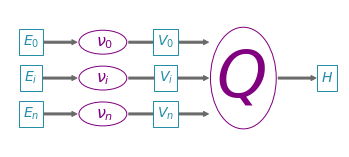
\includegraphics[width=1\textwidth]{../paper/figures/path_of_q.png}
    \end{figure}
\end{frame}

\begin{frame}{Encoding + Assembly Stages}
    %E-V and Q diagram    
\end{frame}
\begin{frame}{Encoding + Assembly}
    \begin{figure}
        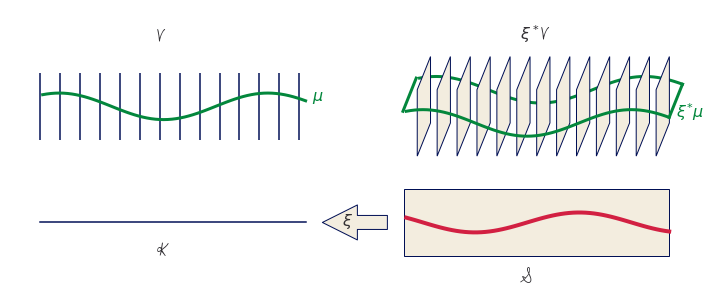
\includegraphics{../paper/figures/q_hat.p}
    \end{figure}
\end{frame}
\begin{frame}{Domain and Range}
    \begin{figure}
        \begin{subfigure}{.5\textwidth}
            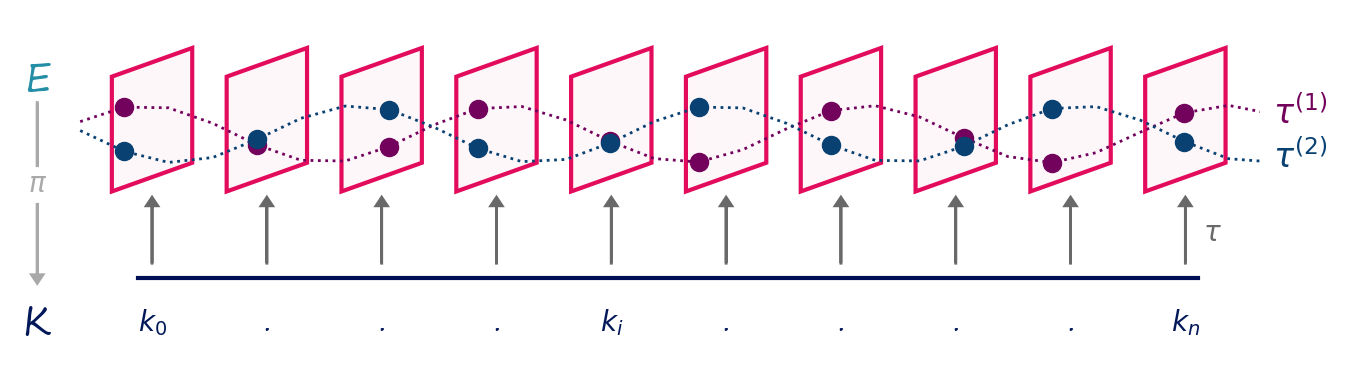
\includegraphics[.5\textwidth]{../paper/figures/fiberbundle.png}
        \end{subfigure}
        \begin{subfigure}{.5\textwidth}
            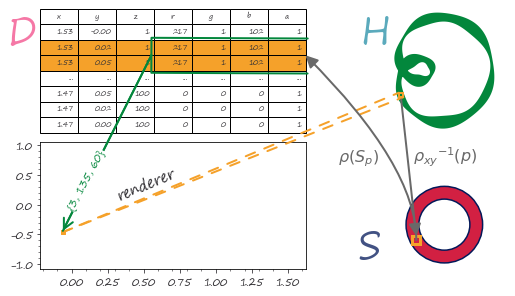
\includegraphics[.5\textwidth]{../paper/figures/render.png}
        \end{subfigure}
    \end{figure}
\end{frame}

\begin{frame}{Example $\dfunctc$: Stevens' Scales \cite{stevensTheoryScalesMeasurement1946}}
\begin{table}[H]
    \begin{tabularx}{\textwidth}{|l|l|X|}\toprule
        \textbf{scale} & \textbf{group} & \textbf{constraint} \\\midrule
        nominal & permutation &  $\text{if } \delement_1 \neq \delement_2 \text{ then } \vchannel (\delement_1) \neq\vchannel(\delement_2)$\\
        ordinal &  monotonic & $\text{if } \delement_1 \leq \delement_2 \text{ then } \vchannel (\delement_1) \leq \vchannel(\delement_2)$\\
        interval &  translation &  $\vchannel (x + c) = \vchannel(x) + c$ \\
        ratio &  scaling &  $\vchannel(xc) = \vchannel(x)*c $\\ \bottomrule
    \end{tabularx}
\end{table}
\end{frame}



\begin{comment}
\begin{frame}{Scatter: $\vmark(xpos, ypos)(\alpha, \beta)$}
    \begin{figure}[H]
        \begin{overprint}
            \onslide<1|handout:0>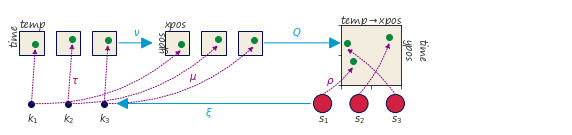
\includegraphics[width=1\linewidth]{figures/math/scatter_q.png}
            \onslide<2|handout:0>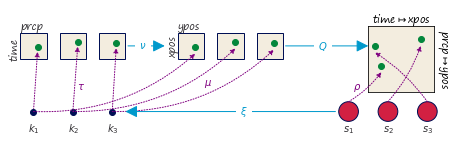
\includegraphics[width=1\linewidth]{figures/math/scatter_with_s.png}
        \end{overprint}
    \end{figure}   
\end{frame}

\begin{frame}{Line: $\vmark(xpos, \hat{n_{1}}, ypos, \hat{n_{2}})(\alpha, \beta)$ }
    \begin{figure}[H]
        \begin{overprint}
            \onslide<1|handout:0>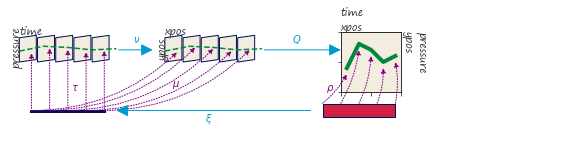
\includegraphics[width=1\linewidth]{figures/math/line_q.png}
            \onslide<2|handout:0>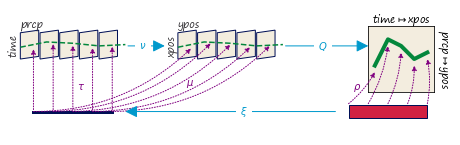
\includegraphics[width=1\linewidth]{figures/math/line_with_s.png}
        \end{overprint}
    \end{figure}   
\end{frame}

\begin{frame}{Image $\vmark(xpos, ypos, color)$}
    \begin{figure}[H]
        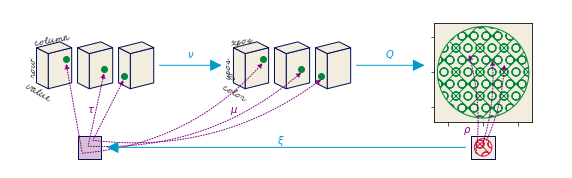
\includegraphics[width=1\textwidth]{figures/math/image.png}
    \end{figure}
\end{frame}

\begin{frame}{Build \vmark\ over \dbase: \vmarkd}
\begin{figure}[H]
    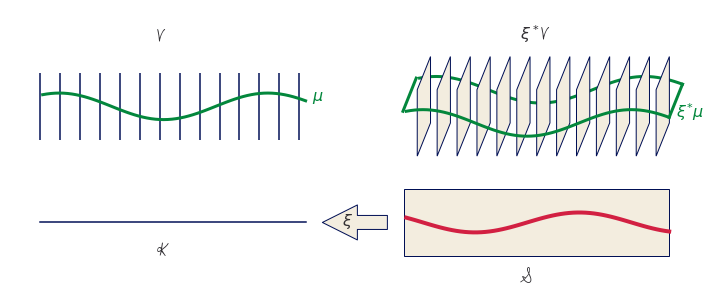
\includegraphics[width=1\textwidth]{figures/math/q_hat.png}
\end{figure}
\begin{equation*}\label{eq:qhat_q_s}
    \vmarkd(\vsection(\dbasepoint))(\gbasepoint) \coloneqq \vmark((\vsectionpull)(\gbasepoint))
\end{equation*} 
\end{frame}

\begin{frame}{Composition of artists $+ \coloneqq \sqcup \dtotal_{i}$} 
    \begin{figure}
        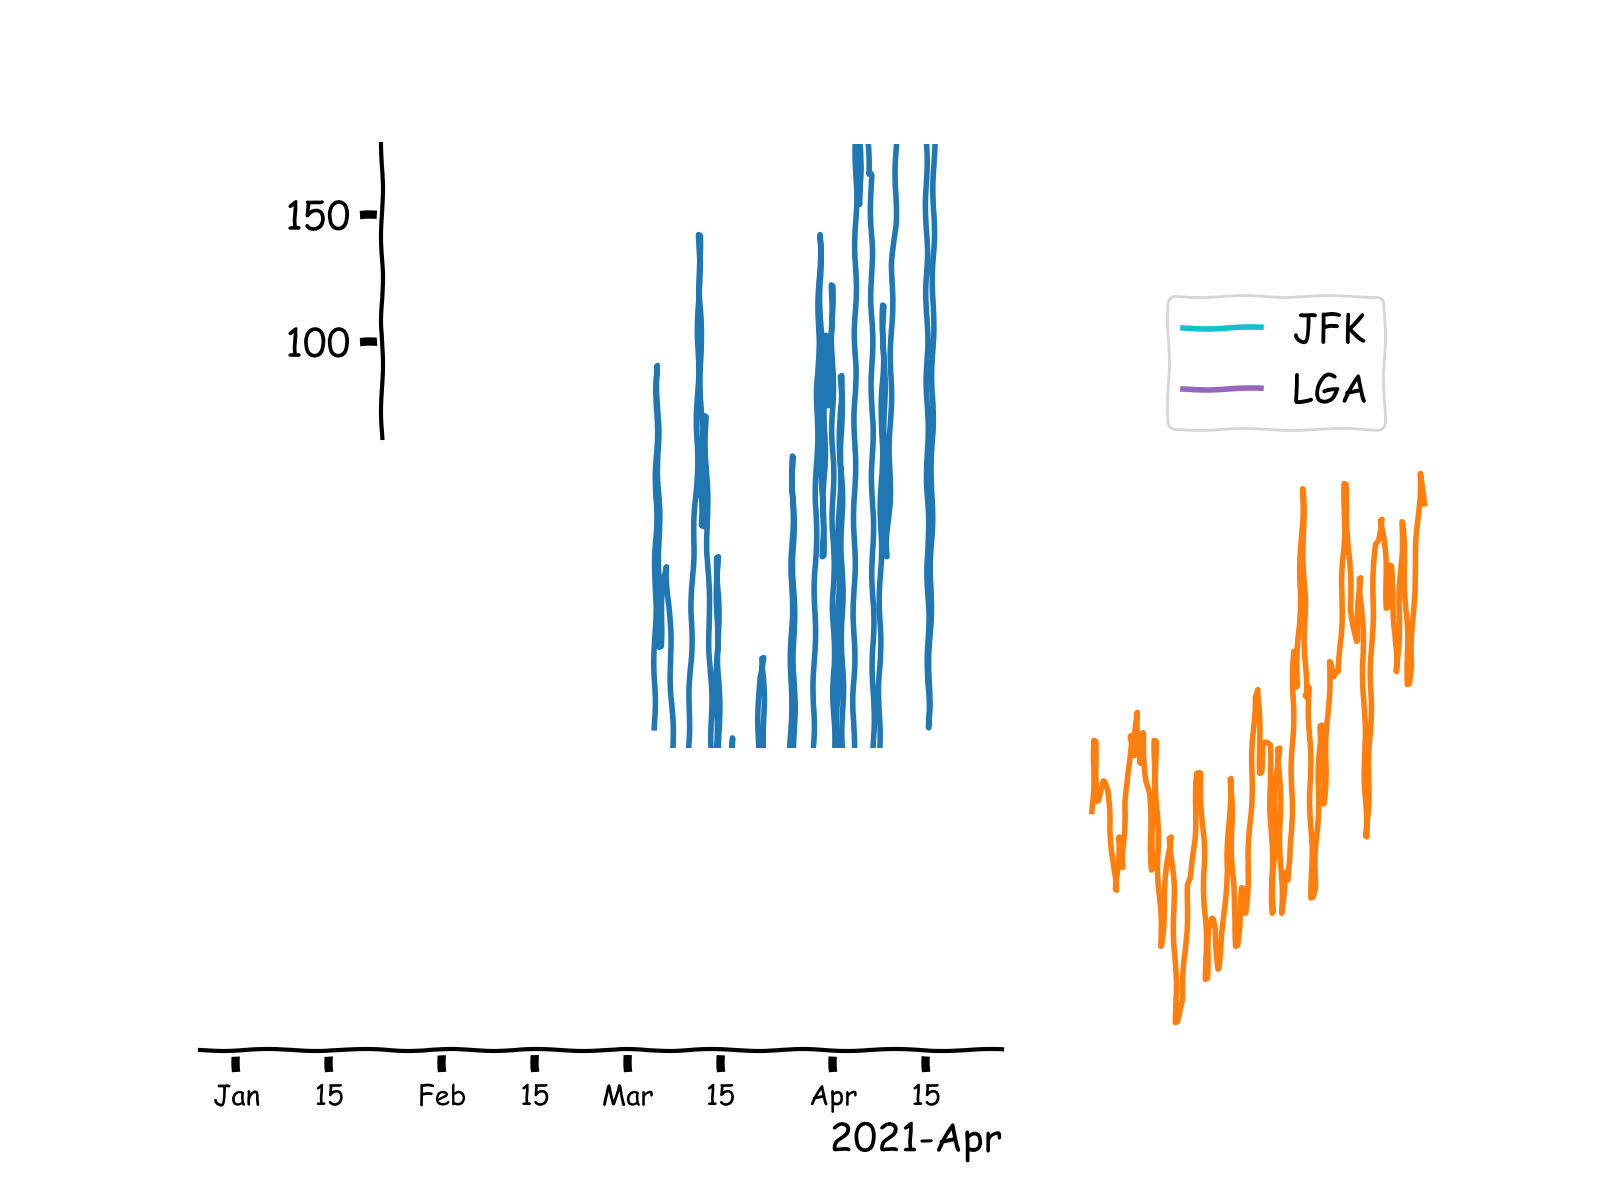
\includegraphics[width=1\textwidth]{figures/math/exploding_artist.png}
    \end{figure}
\end{frame}


\section{Code}
\begin{frame}{TEAM driven rearchitecture of Matplotlib}
    \begin{itemize}
        \item complex visualizations
        \pause 
        \item structure preserving maps from data to visual
        \begin{itemize}
            \item data and graphics have equivalent continuity
            \item properties are equivariant under monoid actions
        \end{itemize}  
        \pause
        \item fiber bundles are an abstraction
        \begin{itemize}
            \item topologically complex heterogenous data 
            \item target display spaces
        \end{itemize}
    \end{itemize}
\end{frame}

\begin{frame}[fragile]{How do we make things?}
    \begin{figure}[H]
        \begin{subfigure}{0.49\textwidth}
            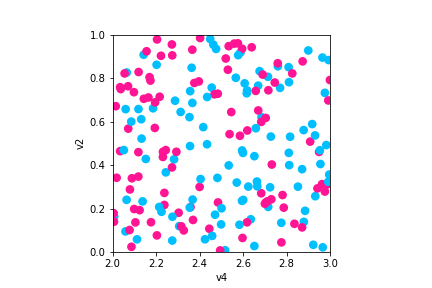
\includegraphics[width=\textwidth]{figures/code/scatter_0.png}
        \end{subfigure}
        \begin{subfigure}{0.49\textwidth}
            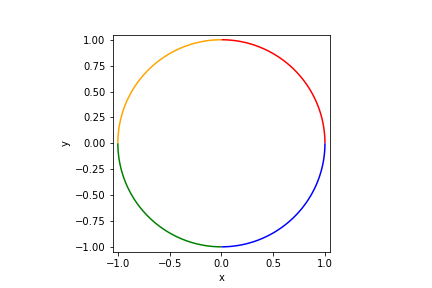
\includegraphics[width=\textwidth]{figures/code/line_1.png}
        \end{subfigure}
    \end{figure}
    \begin{columns}
    \column{0.49\textwidth}
    \begin{minted}{python}
    fig, ax = plt.subplots()
    artist = Point(data, transforms)
    ax.add_artist(artist)
    \end{minted}
    \column{.49\textwidth}
    \begin{minted}{python}
    fig, ax = plt.subplots()
    artist = Line(data, transforms)
    ax.add_artist(artist)
    \end{minted}
    \end{columns}
\end{frame}

\subsection{Artist}
\begin{frame}[fragile]{ \vchannel}
    \begin{minted}{python}
    cmap =  color.Categorical({'true':'deeppink', 'false':'deepskyblue'})
    transforms = {'x': {'name': 'v4', 'encoder': lambda x: x},
                    'y': {'name': 'v2', 'encoder': lambda x: x},
                    'facecolors': {'name':'v3', 'encoder': cmap}, 
                    's':{'name': None , 
                        'encoder': lambda _: itertools.repeat(.02)}}
    \end{minted}
    \begin{itemize}
        \item \mintinline{python}{lambda x: x} is identity \vchannel\
        \item \mintinline{python}|{'name':None}| map into \vfiber\ without corresponding \dsection\
        \item \mintinline{python}{color.Categorical} is custom \vchannel
    \end{itemize}
\end{frame}
    
\begin{frame}[fragile]{\vartist} %% rewrite w/ letters in talk
    \begin{minted}{python}
        class ArtistClass(matplotlib.artist.Artist):
            def __init__(self, E, V, *args, **kwargs):
                # set properties that are specific to the artist
                # stash the input E and V
                super().__init__(*args, **kwargs)
        
            def qhat(self, **args):
                # set the properties of the graphic
        
            def draw(self, renderer):
                # returns tau, indexed on fiber then key 
                tau = self.E.view(self.axes) 
                # visual channel encoding applied fiberwise 
                visual = {p_i: nu_i(tau_i)
                          for p_i, nu_i, tau)i 
                          in zip(self.V, tau)}
                self.qhat(**visual)
                # pass configurations off to the renderer
                super().draw(renderer)
        \end{minted}
\end{frame}

\begin{frame}[fragile]{\vmarkd}
\begin{minted}{python}
    class Point(mcollections.Collection):
        def assemble(self, x, y, s, facecolors='C0' ):
            # construct geometries of the circle glyphs in visual coordinates
            # set attributes of glyphs

    class Line(mcollections.LineCollection):
        def assemble(self, x, y, color='C0'):
            # assemble line marks as set of segments 
    \end{minted}
\end{frame}

\subsection{Data}
\begin{frame}[fragile]{Continuity}
    \begin{minted}{python}
class PointData: 
    # Fiberbundle is consistent across all sections
    FB = FiberBundle({'tables': ['vertex']},  
        {'v1': float, 'v2': str, 'v3': float})
    def tau(self, k):
        return # tau evaluated at one point k

class LineData: 
    FB = FiberBundle({'tables': ['edge']},
                {'x' : float, 'y':  float, 'color':mtypes.Color()})
    def tau(self, k): 
        return # tau evaluated on interval k
    \end{minted}
\end{frame}

\begin{frame}[fragile]{Same Artist, Different \dtotal}
    \begin{figure}[H]
        \begin{subfigure}{0.49\textwidth}
            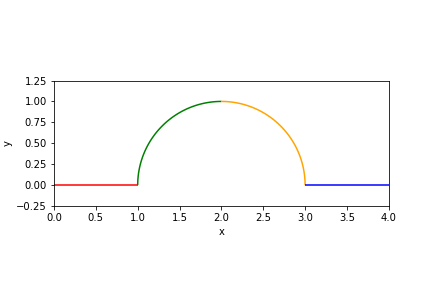
\includegraphics[width=\textwidth]{figures/code/linec_1.png}
        \end{subfigure}
        \begin{subfigure}{0.49\textwidth}
            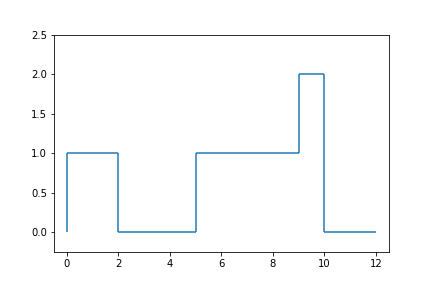
\includegraphics[width=\textwidth]{figures/code/lined_1.png}
        \end{subfigure}
    \end{figure}
\begin{minted}{python}
LineData(FB, edge_table, vertex_table, connect=True)
LineData(FB, edge_table, vertex_table, num_samples=2, connect=False)
\end{minted}
\end{frame}

\begin{frame}{Proposed Work}
\begin{figure}
    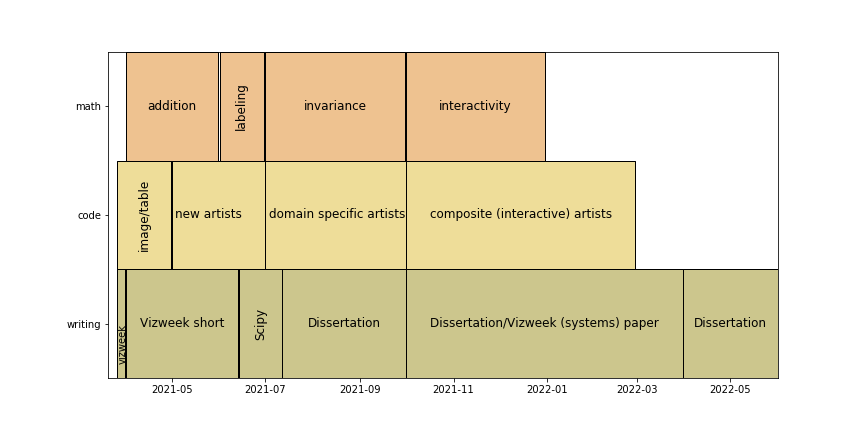
\includegraphics[width=1\textwidth]{figures/intro/gantt.png}
\end{figure}
\end{frame}

\begin{frame}{Acknowledgments}
    \begin{itemize}
        \item Professor Michael Grossberg and Dr. Thomas Caswell
        \item Professor Haralick, Professor Vo, Professor Manovich, Dr. Hanwell
        \item Matplotlib development team 
        \item CZI EOSS (grant number 2019-207333) from the Chan Zuckerberg Initiative DAF, an advised fund of Silicon Valley Community Foundation
    \end{itemize}
    
\end{frame}

\begin{frame}[allowframebreaks]{References}
\printbibliography
\end{frame}
\appendix 

\begin{frame}{Bertin Retinal Variables}
    \begin{figure}
        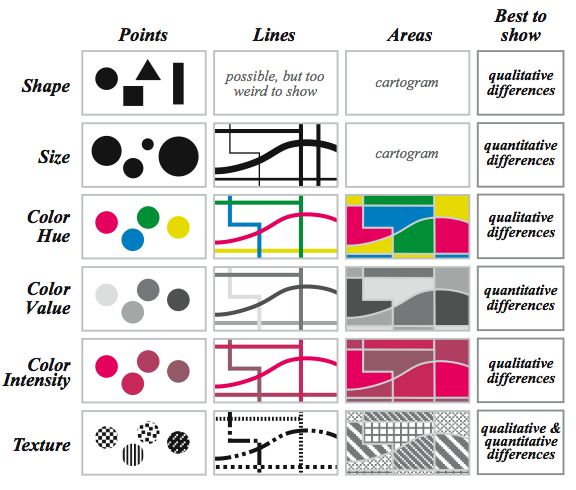
\includegraphics[width=.7\textwidth]{figures/intro/retinal_variables.png}
        \caption{This tabular form of Bertin's retinal variables is from Understanding Graphics \cite{malamedInformationDisplayTips2010} who reproduced it from Krygier and Wood's \textit{Making Maps: A Visual Guide to Map Design for GIS}\cite{krygierMakingMapsVisual2005}}
    \end{figure}
\end{frame}


\begin{frame}{Fiber is all possible values a variable can be \cite{spivakDatabasesAreCategories2010,spivakSIMPLICIALDATABASES}}
    Given a space of all possible values \ftotal\
    \begin{equation*}
        \label{eq:data_types}
        \begin{tikzcd}[ampersand replacement=\&]
            \fttype \arrow[r] \arrow[d, "\pi_{\fsection}"'] \& \ftotal \arrow[d, "\pi"] \\
            \fnames \arrow[r, "\fsection"']                  \& \ftypes       
        \end{tikzcd}
    \end{equation*}
    a fiber component is the restricted space $\ftotal_{\fsection(\fname)}$. 
    \begin{equation*}
        \dfiber = \ftotal_{\fsection(\fname)} = \ftotal_{\ftype} 
    \end{equation*}
    \begin{description}
        \item[\ftypes] data types of the variables in the dataset 
        \item[\ftotal] disjoint union of all values of type $\ftype \in \ftypes$ 
        \item[\fnames] variable names, $\fname \in \fnames$
        \item[\fttype] \ftotal\ restricted to the data type of a named variable   
    \end{description}
\end{frame}

\begin{frame}{Monoid actions}
    A monoid \monoid\ is a set with
    \begin{description}
        \item[associative binary operator] $\ast:\monoid \times \monoid\rightarrow \monoid$
        \item[identity element] $e\in \monoid$ such that $e\ast a= a \ast e = a$ for all $a \in \monoid$. 
    \end{description}
    \begin{block}{left monoid action}
    A set \dfiber\ with an action\cite{nlab:action} $\bullet: \monoid\times \dfiber \rightarrow \dfiber$ with the properties:
        \begin{align*}
            \textbf{associativity}\;& \text{for all } f,g \in \monoid \text{ and } x\in \dfiber,\, f\bullet(g\bullet x) = (f\ast g) \bullet x\\
            \textbf{identity}\;& \text{for all } x\in \dfiber, e\in \monoid,\,  e\bullet x = x 
        \end{align*}
    \end{block}
\end{frame}

\begin{frame}{Keeping track of sections with sheafs}
    Restriction maps of a sheaf describe how local $\iota^*\dsection$ can be glued into larger sections \cite{ghristElementaryAppliedTopology2014,ghristHomologicalAlgebraData2018}
    \begin{equation*}
        \label{eq:sheaf}
        \begin{tikzcd}[ampersand replacement=\&]
            \iota^*\dtotal \arrow[d, "\pi"'] \arrow[r, "\iota^*", hook]             \& \dtotal \arrow[d, "\pi"']                  \\
            U \arrow[r, "\iota", hook] \arrow[u, "\iota^{*}\dsection"', bend right] \& \dbase \arrow[u, "\dsection"', bend right]
        \end{tikzcd}
    \end{equation*}
    The inclusion map $\iota: U \rightarrow \dbase$ pulls \dtotal\ over $U$ such that the pulled back $\iota^*\dsection$ only contains records over $U \subset \dbase$.
\end{frame}

\begin{frame}{Rendering: Define a Pixel}
    \begin{columns}
        \column{0.5\textwidth}
        Given a pixel
        \begin{equation*}
        p=\left[y_{top}, y_{bottom}, x_{right}, x_{left}\right]
        \end{equation*}
        the inverse map of the bounding box 
        \begin{equation*}
        \gbase_{p} ={\gsection_{xy}}^{-1}(p)
        \end{equation*}
        is a region $\gbase_p \subset \gbase$ such that 
        \begin{align}
            \scriptstyle r_p &= \scriptstyle \iint\limits_{S_p} \rho_r(s)ds^{2}\\
            \scriptstyle g_p &= \scriptstyle \iint\limits_{S_p} \rho_g(s)ds^{2}\\
            \scriptstyle  b_p &= \scriptstyle \iint\limits_{S_p} \rho_b(s)ds^{2}
        \end{align}
        yields the color of the pixel. 
        \column{0.5\textwidth}
        \begin{figure}[H]
            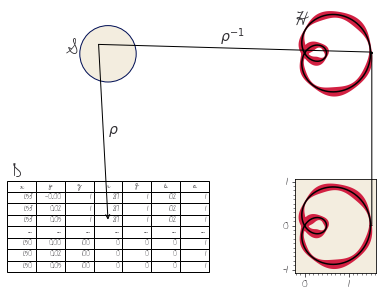
\includegraphics[width=\textwidth]{figures/math/render.png}
        \end{figure}
    \end{columns}
\end{frame}

\begin{frame}{$\mathcal{A}:\mathcal{E}\rightarrow\mathcal{E}$}
    The topological artist is a sheaf map
    \begin{equation*}
    \vartist: \mathcal{O}(\dtotal) \rightarrow \mathcal{O}(\gtotal)
    \end{equation*}
    that carries homomorphism of monoid actions $\varphi: \monoid \rightarrow \monoid^{\prime}$ 
    \cite{cegarraCohomologyMonoidsOperators2019} 
    \begin{equation*}
    \vartist(m\cdot \delement) = \varphi(m)\cdot \vartist(\delement) 
    \end{equation*}
\end{frame}

\begin{frame}{Visual Channel Encoders}
    We define the visual transformers \vchannel\ on components of the data bundle $\dsection_{i}$
    \begin{equation*}
        \label{eq:nu_expanded}
        \{\vchannel_{0}, \ldots, \vchannel_{n}\}: \{\dsection_{0}, \ldots, \dsection_{n}\} \mapsto \{\vsection_{0}, \ldots, \vsection_{n}\}
    \end{equation*}
    as the set of equivariant maps with the constraint 
    \begin{equation*}
        \vchannel_i(m_{\delement}(\dtotal_i)) = \varphi(m_{\delement})(\vchannel_i(\dtotal_i))
    \end{equation*} 
    where $\varphi:\monoid\rightarrow \monoid^{\prime}$ carries a homomorphism of monoid actions. 
\end{frame}

\begin{frame}{\vfiber\ Components}    
\begin{table}[H]
    \renewcommand{\arraystretch}{2}
    \begin{tabulary}{\textwidth}{|l|L|l|}\hline
     $\bm{\vchannel_{i}}$                      & $\bm{\vsection_{i}}$                                                            & $\bm{codomain(\vchannel_{i}) \subset \vfiber_{i}}$  \\ \hline                                              
    position                    & x, y, z, theta, r                                                          & $\mathbb{R}$   \\ \hline
    size                        & linewidth, markersize                                            & $\mathbb{R}^{+}$   \\ \hline
    shape                       & markerstyle                                                      & $\{f_{0}, \ldots, f_{n}\}$ \\ \hline
    color                       & color, facecolor, markerfacecolor, edgecolor  & $\mathbb{R}^{4}$ \\ \hline
    \multirow{2}{*}{texture}    & hatch                                                            & $\mathbb{N}^{10}$\\\cline{2-3}
                                & linestyle                                                        & $(\mathbb{R}, \mathbb{R^+}^{n, n\%2=0})$ \\ \hline              
    \end{tabulary}
    \label{tab:mpl_visual_variable_fiber}
\end{table}
\end{frame}
\begin{frame}{Monoid Equivariance: Partial Orders}
    \begin{figure} %break out steps/reveal
        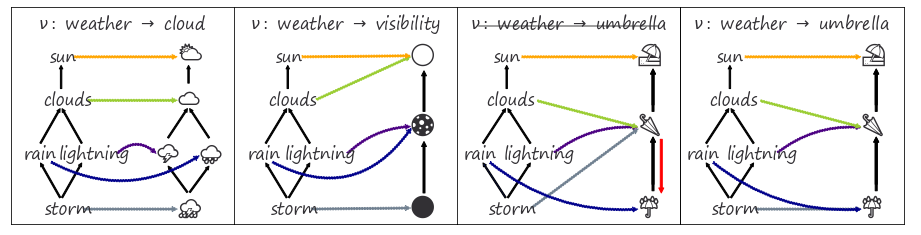
\includegraphics[width=1\textwidth]{figures/math/monoid_equivariant.png}
    \end{figure}
\end{frame}

\begin{frame}{Glyph}
    The glyph is the graphic generated by $\vmark(\gbase_{\dbasepathpoint})$ where the path connected components $\dbasepath \subset \dbase$ are defined 
    \begin{equation*}
    \dbasepath = \{\dbasepathpoint \in \dbase \text{ s. t. } \exists \gamma \text{ s.t. } \gamma(0)=\dbasepoint \text{ and }\gamma(1)=\dbasepathpoint\}
    \end{equation*}
    such that the  path $\gamma$ from \dbasepoint\ to \dbasepathpoint\ is a continuous function from the interval [0,1] and $\gbase_{\dbasepathpoint}$ is the region
    \begin{equation*}
        \begin{tikzcd}[ampersand replacement=\&]
            \gtotal \arrow[r, shift left] \& \gbase_\dbasepathpoint \arrow[rr, "\vindex(\gbasepoint)", shift left] \arrow[l, "\gsection(\gbase_\dbasepathpoint)"] \& \& \dbasepath_{\dbasepoint} \arrow[ll, "\vindex^{-1}(\dbasepath)"]
            \end{tikzcd}
        \label{eq:mark}
    \end{equation*}
    such that the glyph is differentiable, in keeping with Ziemkiewicz and Kosara's description of a glyph\cite{ziemkiewiczEmbeddingInformationVisualization2009}.
\end{frame}

\begin{frame}{Artist Equivalance class}
    When artists share a base space 
    \begin{equation*}
        \dbase_2 \hookrightarrow \dbase_1
    \end{equation*}
    a composition operator can be defined such that the the artists can be considered to be acting on different components of the same section. 
\end{frame}

\begin{frame}[fragile]{Complex \vchannel}
    \begin{minted}{python}
    class Categorical:
        def __init__(self, mapping):
            # check that the conversion is to valid colors
            assert(mcolors.is_color_like(color) for color in mapping.values())
            self._mapping = mapping
    
        def __call__(self, value):
            # convert value to a color
            return [mcolors.to_rgba(self._mapping[v]) for v in values]
    \end{minted}
    That we can test for action equivariance
    \begin{minted}{python}
    def test_nominal(values, encoder):
        m1 = list(zip(values, encoder(values)))
        random.shuffle(values)
        m2 = list(zip(values, encoder(values)))
        assert sorted(m1) == sorted(m2)
    \end{minted}
\end{frame}

\begin{frame}[fragile]{Artist}
    \begin{minted}{python}
        class ArtistClass(matplotlib.artist.Artist):
            def __init__(self, data, transforms, *args, **kwargs):
                # properties that are specific to the graphic
                self.data = data 
                self.transforms = transforms
                super().__init__(*args, **kwargs)
        
            def assemble(self, **args):
                # set the properties of the graphic
        
            def draw(self, renderer):
                # returns K, indexed on fiber then key 
                view = self.data.view(self.axes) 
                # visual channel encoding applied fiberwise 
                visual = {p: t['encoder'](view[t['name']])
                          for p, t in self.transforms.items()}
                self.assemble(**visual)
                # pass configurations off to the renderer
                super().draw(renderer)
        \end{minted}
\end{frame}


\begin{frame}[fragile]{Artists: Scatter \& Line}
\begin{minted}{python}
class Point(mcollections.Collection):
    def assemble(self, x, y, s, facecolors='C0' ):
        # construct geometries of the circle glyphs in visual coordinates
        self._paths = [mpath.Path.circle(center=(xi,yi), radius=si) 
                    for (xi, yi, si) in zip(x, y, s)] 
        # set attributes of glyphs, these are vectorized 
        # circles and facecolors are lists of the same size
        self.set_facecolors(facecolors)

class Line(mcollections.LineCollection):
    def assemble(self, x, y, color='C0'):
        #assemble line marks as set of segments 
        segments = [np.vstack((vx, vy)).T for vx, vy in zip(x, y)]
        self.set_segments(segments)
        self.set_color(color)
\end{minted}
\end{frame}


\begin{frame}[fragile]{View}
\begin{minted}{python}
def view(self, axes):
    table = defaultdict(list)
    for k in self.keys:
        table['index'].append(k)
        for (name, value) in zip(self.FB.fiber.keys(), self.tau(k)[1]):
            table[name].append(value)
    return table
\end{minted}
\begin{description}
    \item [\mintinline{python}{VertexSimplex}] (name, value), value is scaler
    \item [\mintinline{python}{EdgeSimplex}]  (name, value), value is [x0, ..., xn]
\end{description}
\end{frame}

\begin{frame}[fragile]{Fiber Bundle}
    \begin{minted}{python}
    @dataclass
    class FiberBundle:
    """
    Attributes
    ----------
    K: {'tables': []}
    F: {variable name: type}
    """
        K: dict 
        F: dict
    \end{minted}
\end{frame}

\begin{frame}[fragile]{GraphLine Data Model}
\begin{minted}{python}
class GraphLine:
    def __init__(self, FB, edge_table, vertex_table, num_samples=1000,
                        connect=False):
        #set args as attributes and generate distance
        if connect: # test connectivity if edges are continuous
            assert edge_table.keys() == self.FB.F.keys()
            assert is_continuous(vertex_table)

    def tau(self, k):
        # evaluates functions defined in edge table
        return(k, (self.edges[c][k](self.distances) 
                        for c in self.FB.F.keys()))

    def view(self, axes):
        # walk the edge_vertex table to return the edge function
        table = defaultdict(list)
        for (i, (start, end)) in sorted(zip(self.ids, self.vertices), 
                                            key=lambda v:v[1][0]):
            table['index'].append(i)
            # same as view for line, returns nested list
            for (name, value) in zip(self.FB.F.keys(), self.tau(i)[1]):
                table[name].append(value)
        return table
\end{minted}
\end{frame}
\end{comment}
\end{document}

